\chapter{Software Design}
\label{sec:ch3_soft}
This section outlines the design methodology for the SHARC Buoy Software. The software cycle was designed with consideration towards the IEEE software standard 12207.1\footnotetext{Software life cycle processes—Life cycle data\cite{IEE_STD_SOFTCYCLE}}.


The software structure was kept as compartmentalised as possible to improve the modulator of the firmware. This would allow for fewer changes to be made during the design process allowing for a quick response to hardware changes. The design process was iterative as changes were made over the design cycle to the micro-controller platform as well as the sensors. In addition, some of the required libraries had depreciated and needed to be replaced.  This section will focus solely on the firmware design for the overall system as well as the subsystem. 

This section begins with an overview of the development environment which discusses the tools, platform and any libraries that were used. Then an overview of the main firmware is given. Each aspect of the system is described in terms of function, configuration parameters as well as location in the overall scope.

\section{Software Architecture}

The STM32 series does not come loaded with any Operating System. Therefore, firmware development had to occur on bare metal. In addition, the firmware had to be tailored to the specific micro-controllers architecture. The Atollic Truestudio IDE allowed for development to take place in C. The program comes packaged with an ARM development tool chain and a C compiler allowing for code to be compiled and flashed onto the board via a USB cable. The manufacturer also provides a set of driver files and  initialisation tools. The project was written in C which allowed for higher-level code to implemented while still optimising for size and speed on the device. In addition, C allows for the program to include drivers and resources from the manufacturer. \par 

The Firmware was designed using a top down approach. The overall system was decomposed into 3 distinct layers as shown in the figure below

\begin{figure}[H]
	\centering
	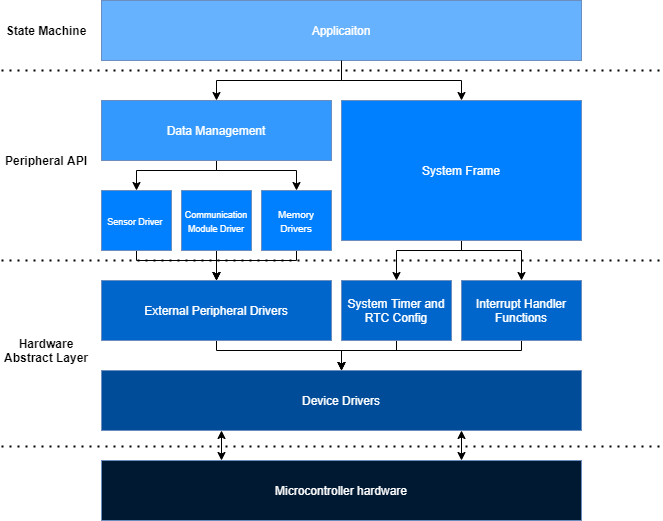
\includegraphics[width= 0.7\linewidth]{soft_arch.png}
	\caption{Diagram showing the decomposition of the overall firmware into distinct layers and the relationship between each part.}
	\label{fig:soft_arch}
\end{figure}

The Hardware Abstract layer consists of the driver files used to initialise and control the hardware of the micro-controller.This layer is platform specific therefore needs to be tailored to the architecture of the micro-controller. The manufacturer provides hardware driver files which were used to form the Hardware abstract Layer.The Standard Peripheral Library (SPL) was used in the first version of the firmware however, the library had depreciated and was replaced with the Hardware Abstract Layer (HAL) libraries. HAL libraries were used to form the foundation of the code as it allows for the code functionality to run independently from the hardware architecture. Should a new micro-controller be required, the HAL library simply needs to replaced. Therefore allowing the firmware to maintain modularity and increase portability. In addition, the HAL Library offers robust error checking and flagging. If a peripheral fails at any point during run time, the libraries provide handlers and flag signalling to handler the error. \par 
Once The HAL Layer was finished, customised driver files were written for each module. These files were written to interface with the sensor through the HAL layer thereby reducing dependencies on the hardware, in addition, these driver files were created to abstract the initialisation and configuration process of each peripheral as well as the hardware routines that occur. In addition, some external modules required the use of more than one peripheral such as timer channels for input capture or GPIO pins for External interrupt detection. Finally, these drivers are critical for managing the flow of data too and from the module. The files contain functions that interpret incoming data bytes and convert them to the relevant data type.

\par 

Finally, driver files, configuration files and other libraries are synthesised and sequenced into one main program. This program calls the functions defined in the Driver files. This program provides a frame for the various modules to interact with system. This will be discussed in greater detail in the section below

\section{Project Structure}

The project was set up using CUBEMX for creating peripheral initialization and handling functions. Final code for the project can be found in the folder BUOY\_Frame\_L4. All the tools, definitions and functions developed for the Buoy frame have been organised into the library files Sharc\_Frame.h and Sharc\_Frame.c. This allows for the frame to ported over multiple projects allowing for a new firmware version to be developed from scratch instantly.
The project code files are organised into the following folders:

\begin{enumerate}
	\item Drivers
	\item src
	\item Start Up
\end{enumerate}
The project code files are organised into the following folders:
1.	Drivers 
2.	SRC
3.	Start Up
The Drivers folder contains the HAL and CMSIS libraries for the device.  The SRC Folder contains the main.c file which acts as the entry point for the program to run. The start up file contains assembly code that specifies the vector table, Hard fault/ Reset Handler Entry Points as well as the entry point for the main code. When the file startup\_stm32l476xx.s is run, the program enters into the main() function and begins running from there. The SRC folder contains the .h/.c pair Sharc\_Frame files which are implemented in the main.c 
The main() code consists of a set up phase and a loop phase. During the set-up, the functions HAL\_Init(); and SystemClock\_Config(); are used to reset the peripherals and the systick timer and set the System clock to the correct source and speed. These two functions run in the set-up phase of the code and are called whenever the program re-enters the main function. The next step in the set up phase is to configure the unused GPIO pins to analog floating mode. This greatly reduces the current consumption by the micro controller. The peripherals required for debugging the code are placed here. Before deployment, the code will be removed. This phase is referred to in the program as the System Init and Clock Configuration. It is the first phase to be run.
The next phase in the Set-up is the Power and Reset State Check. If any power event occurs, a software reset is generated, and the program will restart from the main() function. When this happens, a flag is set in the RCC\_CSR. This can occur in the form of a brown out, Pin reset or Low Power event. This phase will check for the occurrence of any event and handle them before the program enters the main loop. Finally, if successful the program will enter the main loop and the firmware will begin.  

\subsection{Power Mode Selection}

The focus on development optimizing for power consumption as well as accuracy. The system requirements are extremely flexible since the required sampling rate is very slow for example, the largest consideration of the system is Accelerometer sensing which has a maximum expected sample rate of 100Hz. For this reason, high speed computing techniques are not required and do not require much optimization. Since the system will most likely be in a wait state for the majority of its operation, It is important to place the device in as low power mode as possible to minimize consumption. This will be elaborated on in the following sections
The biggest Consideration with system operation is clock speed and source. The STM32l4 has 5 possible options: 3 internal oscillators (MSI,LSI,HSI) and 2 external crystal oscillators (HSE and LSE) these clock sources will provide power to the peripherals as well as the RTC. According the reference manual, the real time clock must be clocked from the LSE 32.768KHz crystal in order to provide an accurate calendar function therefore, the RTC must be clocked from the LSE no exceptions. The external crystal oscillators provide high precision clock speed with extremely low drift however, the power consumption of these oscillators are much higher than the internal RC. The clock configuration of the STM32L4 allows for a combination of these oscillators in a Phase Locked Loop (PLL) which allows for a greater degree of accuracy at desired speeds. 

\begin{figure}[H]
	\centering
	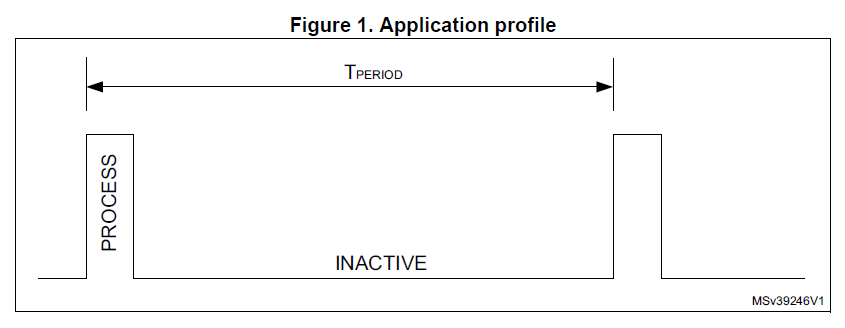
\includegraphics[scale= 0.6]{Application profile.png}
	\caption{Diagram showing a general low power operation profile  for the micro controller with two distinct phases: Process and Inactive occuring over a period T}
	\label{fig:appr}
\end{figure}

Figure \ref{fig:appr}

above details a typical low power operation Which can be expected from the buoy For a typical application, we consider two main phase:
\begin{enumerate}
	\item Process phase: System is in run mode with peripherals are active at regular intervals.
	\item Inactive phase: System is asleep until RTC/GPIO event.
\end{enumerate}

Once the buoy has finished an active routine, the system becomes inactive between samples. The buoy is designed to operate in routines occurring once every half an hour. Once the routine is complete, it still has to wait an extremely long time before it is required again. This is the inactive between sample mode and consider this our period of inactivity where we can place the device in the lowest possible state with very little concern for wake-up time or peripheral settings. \par 
Therefore, the following power modes were selected for each phase of the system's operation

\begin{table}[H]
	\centering
	\caption{Table showing the power mode selection for each phase of the Buoy's operational cycle}
	\begin{tabular}{|c|c|c|}
		\hline 
		Phase &  Power Mode & Current Draw \\
		\hline
		Process & Run Mode & 1.16mA\\
		Inactive & Standby Mode & 710nA\\
		\hline
	\end{tabular}
	
	\label{tab:powmode_cycle}
\end{table}

Table \ref{tab:powmode_cycle} above shows the estimated current consumption taken from the STM32L4 datasheet. The Current Value for Run Mode was bench-marked using a Dhrystone Test with an system clock of 24MHz and code loaded from Flash. The Inactive current draw was estimated with a Low Speed External Oscillator supplying the Real Time Clock. 

\subsection{Clock Selection}

The biggest Consideration with system operation is clock speed and source. The STM32l4 has 5 possible options: 3 internal oscillators (MSI,LSI,HSI) and 2 external crystal oscillators (HSE and LSE). Since the buoy will be inactive for long periods of time, an accurate 1Hz reference signal is required to keep calendar date and time. In addition, The STM32 microcontroller features a variety of wake up options to transition from low power mode to run mode
\begin{enumerate}
	\item Internal  configurable Alarm
	\item Periodic Wake Up Alarm
	\item External Wake Up Pin
\end{enumerate}

These options are made available through an internal Real Time Clock on the STM32L4 microcontroller. The peripheral can receive input from multiple clock sources such as an external Low Speed Oscillator (LSE), an internal Low Speed Oscillator (LSI) or an internal High-speed Oscillator (HSI). The peripheral also allows for fast and simple data storage during extreme power down modes. When the device enters shutdown mode, RAM is turned off, therefore all data will be lost. The RTC has 32 back up registers capable of retaining 1Kb of data when the device is powered down. \par 

these clock sources will provide power to the peripherals as well as  According the reference manual, the real time clock must be clocked from the LSE 32.768KHz crystal in order to provide an accurate calendar function therefore, the RTC must be clocked from the LSE no exceptions. The external crystal oscillators provide high precision clock speed with extremely low drift however, the power consumption of these oscillators are much higher than the internal RC. The clock configuration of the STM32L4 allows for a combination of these oscillators in a phase locked loop (PLL) which allows for a greater degree of accuracy at desired speeds. The final clock configuration parameters are shown in the table below:

\begin{table}[H]
	\centering
	\caption{configuration parameters for the system clock and Real Time Clock including sources and frequencies}
	\begin{tabular}{|l|l|}
		\hline
		Run Mode System Clock Source: & MSI and LSE in a PLL Configuration \\
		\hline
		Clock Frequency: & 24 MHz \\
		\hline
		Shut Down Mode Clock Source: & LSE \\
		\hline 
		RTC Clock Frequency & 1 Hz \\
		\hline 
		LSE Clock Frequency  & 32.768 KHz \\
		\hline 
	\end{tabular}
	\label{tab:clock_conf}
\end{table}

\section{Firmware Overview}

In a multi-sensing system, it is important to manage the interactions and data flow between the various aspects of the system to ensure the device operates in a predictable, manage manor. To achieve this, a state machine can be implemented to provide a high-level form of control over the system. This can be achieved by decomposing the overall function of the buoy into a series of finite states. These states are connected through a series of transitions which can be described using Boolean techniques. Through this, the buoy retains a modular structure both in firmware and in hardware which can allow for additionally sensors and functions to be implemented seamlessly.\par 


\subsection{Execution}

The goal of the buoy is to sample environmental, GPS and power data at a fixed rate. This rate $T_{sample}$ will be used to describe the period between sampling the devices. Each Sample will be condensed into a byte packet and stored in flash memory at a sector. After every 4 samples, the device will load the packets from memory into a buffer and transmit the data. When the device exits this state, it will reset the sample count and repeat until the buoy is turned off or loses power. The buoy can therefore be broken down into a set of finite states which are shown below:

\begin{enumerate}
	\item \textbf{Initialisation State:} The device initializes the counter and verifies the sensors.
	\item \textbf{Reset State:} Counter and memory Variables are Reset
	\item \textbf{Sample State:} During this state, the device actively receives data from the sensors and stores them into a packet which is then saved to Memory
	\item \textbf{Sleep State:} The device enters this state between samples and active states. Here, the device will remain in this state for a time $T_{sample}$. After which, the buoy will wake up 
	\item \textbf{Transmit State:} The device will load the data from memory and transfer to the Iridium Modem Buffer. Upon successful transmission, it will enter the Reset state
\end{enumerate}

Each state will control which routines are performed during the function and provide the system with information on the current status of the device. Should the device encounter a hardware reset, the system can recover and predict the action it needs to take based on the last state the system was in. A typical system run is shown in the figure below:

\begin{figure}[H]
	\centering
	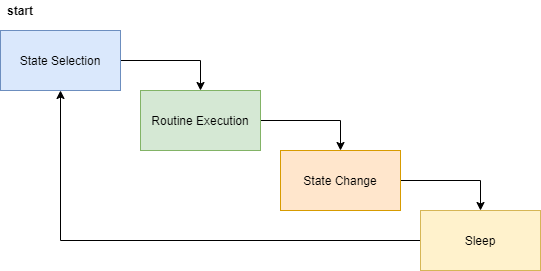
\includegraphics[scale = 0.5]{state Run.png}
	\caption{Diagram showing the steps executed from wake up when }
	\label{fig:state_run}
\end{figure}

The inputs to the state machine are:
\begin{enumerate}
	\item C: a 2-bit integer signifying the number of samples performed $(0 \leq N <4)$
	\item T: Variable that matters when the system is asleep. Signifies whether the system has been in sleep mode for a time defined by the constant value $T_{wake}$
\end{enumerate}

The system has no explicit outputs however, the state machine is used to control which routines will be executed during the execution phase of the program. Therefore, the outputs can be considered as the Routine Rx as shown below:
\begin{enumerate}
	\item $R_{sample}$: Sensor sample routine, this can involve all the sensors or just a select number. For simplicity's sake, this period implies all sensors will be sampled from
	\item $R_{sleep}$ : Device is in a sleep state and will wake up when the periodic wake up unit counts to a time $T_{wake}$
	\item $R_{Transmit}$ : Satellite Transmission Routine
\end{enumerate}

Given the following information, the Algorythmic State Machine (ASM) chart is derived and shown in the figure below

\begin{figure}[H]
	\centering
	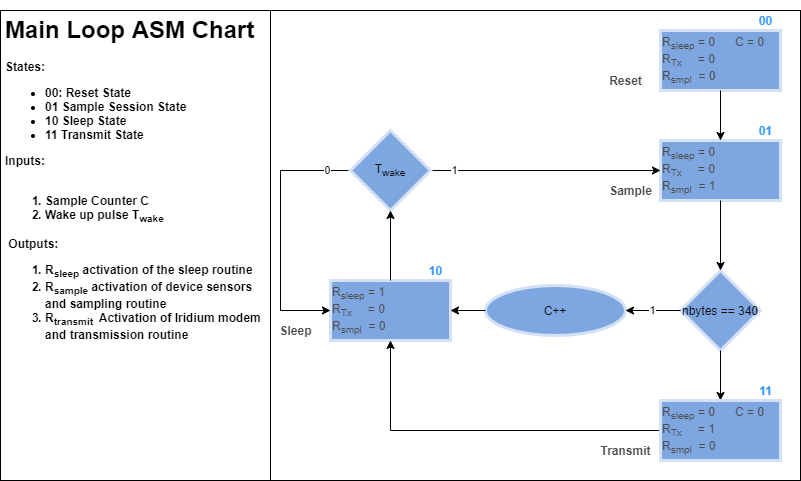
\includegraphics[scale=0.6]{Main Loop ASM Chart.png}
	\caption{ASM chart for the proposed program to run on the processor showing entry/exit conditions and functions to be run during states.}
	\label{fig:ASM_chart}
\end{figure}

Figure \ref{fig:ASM_chart} above shows an abstract representation of the logical flow of the program. A typical run from the system will have the buoy initialised and calibrated before entering the main loop where it will alternate between active sampling and inactive sleep mode until enough data has been collected to transmit. This allows the Iridium modem to only be turned on when needed thereby significantly conserving energy while allowing for the system to sample as much as possible. The variable $T_{wake}$ is user defined and sets the sample rate of the system For this application it has been set to 30 minutes. The device will sample 4 times with 30 minute intervals in-between and transmit the data on the 4th cycle i.e. every 2 hours.

The RTC periodic wake up unit is used as a counter in deep sleep mode. This is a 16-bit down-counting Auto Reload Register that generates an interrupt on an internal wake up line when the system has Slept for a length of time T as defined by the user. In addition, the sample counter gets reset after every transmission state and when the buoy enters a reset state. The number of samples before transmission is chosen to be 4 to optimize packet size for the transmission buffer. Since the Iridium Buffer is 340 Bytes long and the Transmission rate is per 50 bytes, the goal is to transmit as much data that would fit into the buffer as possible. Too frequent transmissions incur a high data cost but result in data integrity. Too few transmissions can result in lost sample points if a transmission is not received.

\subsection{Asynchronous Behaviours}
Asynchronous behavior describes all functionality that occurs outside of the main loop. This can come from Interrupts/ External events which causes the system to exit the main loop regardless of state and execute the code. This can occur from the following sources:

\begin{enumerate}
	\item Interrupts
	\begin{enumerate}
		\item Iridium Message Received (Ring Alert)
		\item IMU Event Detection (Collision / Free-fall detection)
	\end{enumerate}
	\item Events
	\begin{enumerate}
		\item Low power detection.
		\item Brown out detection.
		\item Software resets.
		\item Watch Dog resets.
	\end{enumerate}
\end{enumerate}

These events take precedence over the main loop function. The table below shows the entry/exit conditions. Functionality as well as return state after exit. A full description of events, interrupts, and the protocols for handling them are shown in tables \ref{tab:Int_desc_RI} to \ref{tab:Ev_desc_SWR} in Appendix \ref{sec:evt}. The figure below shows how the event handling procedure is sequenced in the main program:

\begin{figure}[H]
	\centering
	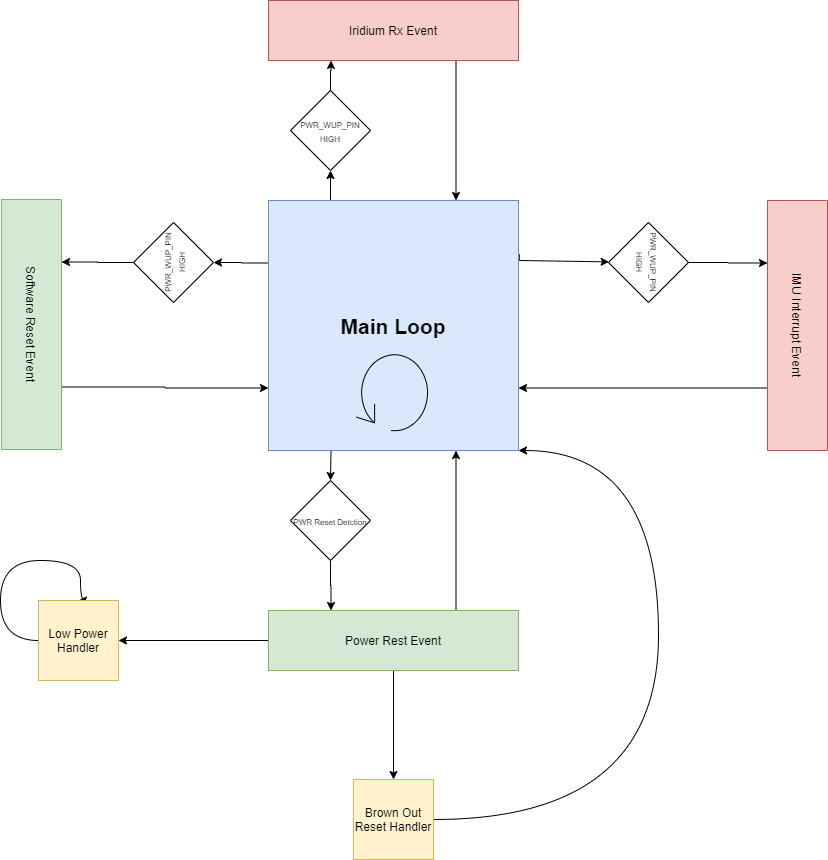
\includegraphics[scale=0.4]{Asynchronous State diagram.png}
	\caption{Application Diagram with Event and Interrupt sequencing}
	\label{fig:main software}
\end{figure}

States are represented by integers on the system and are stored in the back up registers of the RTC. These registers keep data even when the device is in low power mode or a software reset has occurred therefore making them the perfect storage location. The State Variable holds the value of the current state of the buoy. This variable is stored in two locations: When the system is in run mode, the value is stored in the global variable \textit{Current\_State}. When the device is in a deep sleep state, The variable is stored in the RTC Back up registers at byte 0 of Back-Up Register 0. Upon wake up, the value is loaded from the register and placed in the global variable.

The main loop follows a sequential state transition as described in Figure \ref{fig:main software}. To achieve this, at the start of each loop, the program reads the value stored in the state variable. This determines what the previous state was. Based on this value, the new state is determined and stored in the state variable. This process is shown in the figure below.

\begin{figure}[H]
	\centering
	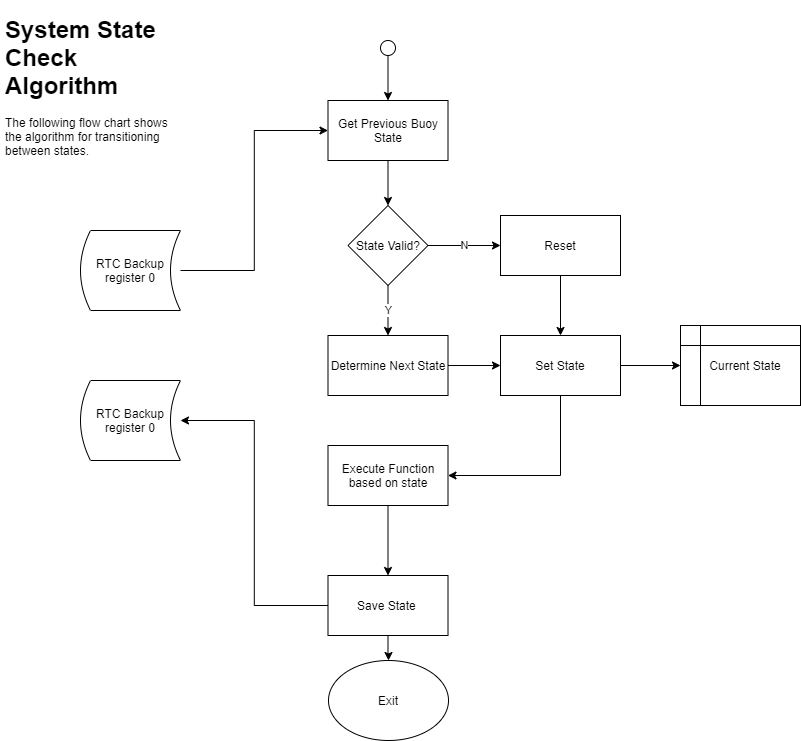
\includegraphics[scale=0.5]{State Check Algorithm.png}
	\caption{Flow chart for the state-check algorithm}
	\label{fig:state_check}
\end{figure}

Figure \ref{fig:state_check} above shows the algorithm for selecting and transitioning between states. This algorithm allows for states to be linked in any order and, most importantly, Separates the state selection from the state function. By separating these two concepts, a more modular framework is created. This allows for the addition of more states and transitions without modifying the routines that are currently in place. This allows for device functions to be turned on and off as desired without drastic changes to the firmware.

Finally, Asynchronous States take a higher precedence over the main loop states and therefore are checked before the state check shown above. The order of precedence is shown in the table below:
\begin{table}[H]
	\centering
	\caption{Table showing the types of states that the system checks for ordered by priority with 1 being the highest priority and 3 being the lowest}
	\begin{tabular}{|l|c|}
		\hline
		Name & Priority \\
		\hline
		Power Event & 1 \\
		\hline
		Asynchronous Interrupt & 2 \\
		\hline
		Sequential State & 3 \\
		\hline
	\end{tabular}
	
	\label{tab:state_prio}
\end{table}

Power Events generate a system reset and raise a flag in the PWR Status Register. When the flag is set, the program enters the handler and, if the event is non-fatal, returns to the main loop. The following flow chart shows an example of such a case for a Brown Out Event

\begin{figure}[H]
	\centering
	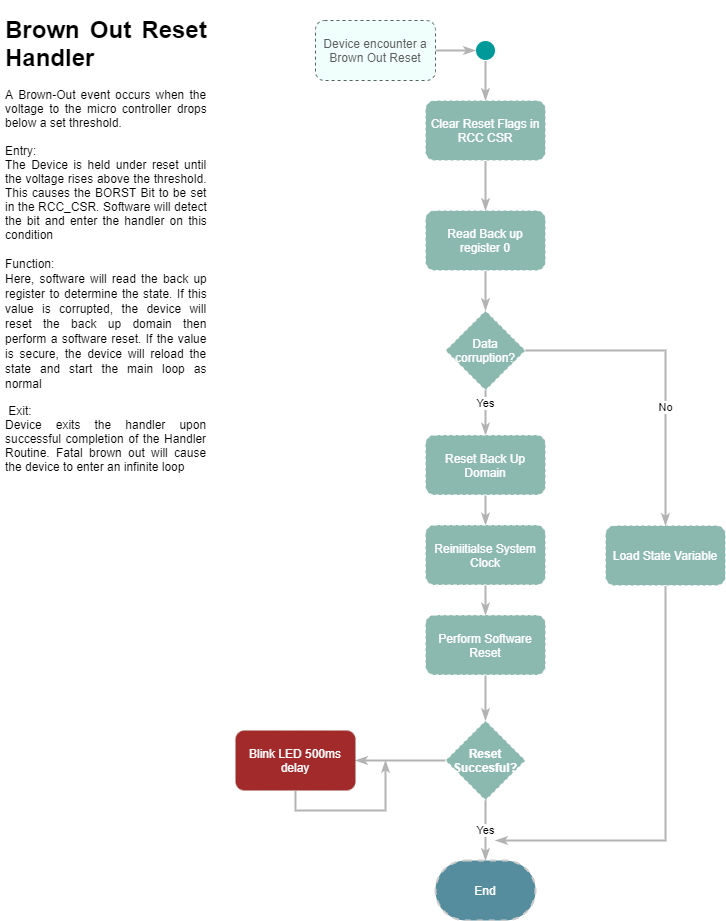
\includegraphics[scale = 0.4]{Brown Out Reset Handler Flow Chart.png}
	\caption{Diagram showing the algorithm for Brown Out Event Recovery and Handling}
	\label{fig:evt_handle}
\end{figure}

Some sensors have interrupt pins and can be configured to trigger upon detection of a specific event. When this happens, the sensor will send a digital high on the interrupt pin. On the processor side, a hardware interrupt is generated and the software handles the interrupt. An example of such a prceedure is shown in the figure below

\begin{figure}[H]
	\centering
	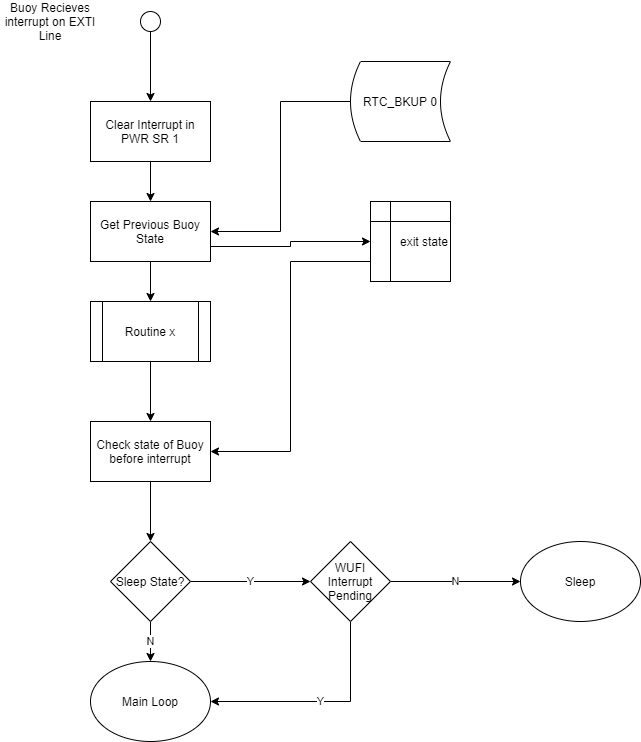
\includegraphics[scale = 0.5]{Asynchronous State flow chart.png}
	\caption{Diagram showing the algorithm for handling an external interrupt from a Wake Up pin connected to one of the modules}
	\label{fig:int_handle}
\end{figure}

By connecting these pins to external wake up pins, the buoy is capable of event detection in deep sleep mode. If an event is detected while in deep sleep, the interrupt causes the buoy to wake up and resume from the beginning. No interrupt handler is entered at this point. A flag is set the PWR\_SR at the position of the wake-up pin it detected. The buoy will enter the asynchronous state depending on which flag is set and will execute the routine associated with it.  When the buoy wakes up from an internal wake up timer, the pins are reconfigured into GPIO EXTI mode which allows the buoy to receive interrupts when active. Note: by keeping the buoys configured as wake up pins, the system will reset when an interrupt is detected.

\subsection{Subsystem Execution}

When a module is is being used at any point in the program. The micro-controller will execute an initialise routine. This will enable any required peripherals for communication with the subsystem. This function will be called before every sample period in case the system encounters a power surge or an unexpected reset. Additionally, placing the micro controller in deep sleep mode results in the registers being reset upon wake up. The initialisation routine is specific to each micro-controller and includes the following:

\begin{enumerate}
	\item High Level Communication Peripheral Configuration
	\item Low Level Pin configuration
	\item Sensor Verification function
	\item Sensor Configuration function
	\item Return Status
\end{enumerate}

The outcome of the initialisation routine is evaluated based on a return status from the function. Items 1 - 3 are included to configure the subsystem to adhere to the functional requirements in table \ref{tab:sys_specs}. Sensor Verification functions are included to satisfy acceptance Tests AT001 and provide evaluations for acceptance tests AT002 and AT004. The initialisation function is designed handle fail modes by evaluating the system's failure return type and responding in accordance with the protocols outlines in acceptance Test 2. Initialisation routines for each subsystem is provided in Appendix \ref{fig:Init_diagram_gps} to \ref{fig:Init_diagram_mpu}

If the initialisation was successful, the program will continue using the module in the firmware. Should a failure occur, the system will attempt to reconnect with the device a predefined number of times. In case of a critical failure, the system will acknowledge that it can no longer use the device and will continue the main firmware without it. The resulting behaviour is shown in the table below:

\begin{table}[H]
	\centering
	\caption{Table Showing the device behaviour in case of a critical failure in one or more of the subsystems. Critical failures are defined in AT006 (table \ref{tab:AT006}) testing protocol.}
	\begin{tabular}{|l|l|l|}
		\hline
		\textbf{Device Failure Case:}  & \textbf{Impact:} & \textbf{Result:}\\
		\hline
		Iridium & Critical & No data will be transmitted from the buoy \\
		\hline
		Flash Chips & Critical & Data will be lost when power is reset \\
		\hline
		GPS & High & GPS data will not be captured \\
		\hline
		MPU6050 & High & Unable to measure Waves in Ice  \\
		\hline
		Environment Sensor & Medium & Environmental data will not be captured \\
		\hline
		Power Monitor & Low & Current and voltage measurements will not be captured \\
		\hline
	\end{tabular}
	\label{tab:exe_subsy_Failiure}
\end{table}
\section{Data Management}

A critical consideration for the system is the flow of data and memory Management. The flash chips provide a solution for permanent storage however, it is critical that data integrity be maintained.Some form of data organization must be implemented for intelligent retrieval/ storage of data in a meaningful way. In addition, the system requires some form of back up should the device be unable to connect to the flash chips. \par 

The flash Chips being used are AT45DB641E SPI Serial Flash Chips. Each chip can hold up to 64Mbit of data. Data can be read/ written at speeds of up to 85MHz of 15MHz in low power mode. The device is low power with high data retention requiring a supply voltage of 1.7V – 3.6V and draws a maximum of 11mA in Active Read mode thereby making it one of the lowest power consumption components in the system. In addition, the device comes with 2 x 256byte buffers that can store data while a read/ write operation is taking place. Memory is Organized into sectors (2 – 256 Kbs long), blocks (2kB long) and pages (256 bytes) with write, read and erase options at each level. \par 

In this section, the data requirements from each sensor is listed. The optimal storage strategy is to convert the measurements into binary data and store as an array of bytes at known locations in an array. The data requirements for each component is listed below

\subsection{Drift Data Acquisition}
This section describes how data is aquired from the sensors to form an Ice Drift measurement. Readings are taken from the GPS and environmental sensor with the power monitor being sampled to provide an update on the buoys performance.\par 

The GPS is sampled 4 times over a given interval. The interval between samples can range from 15 minutes to 30 minutes. At each sample point, the following data is recorded

\begin{enumerate}
	\item Time and Date Information
	\item Geographical Coordinates
	\item Dilation of Precision
	\item Diagnostic Information
\end{enumerate}

%Time and Date information 
By Default, the Ublox Neo GPS series uses the National Marine Electronic Standards (NMEA) \footnote{Information about NMEA messaging on the UBlox Neo GPS is taken from the Interface description here: \url{https://www.u-blox.com/sites/default/files/NEO-M9N_Interfacedescription_\%28UBX-19035940\%29.pdf}} format to send messages. This message structure can vary depending on the type of message being sent/ received however, these message follow the same format:

\begin{table}[H]
	\centering
	\caption{ Breakdown of a typical NMEA message string with fields indicating start/stop sequences and character information.}
	\begin{tabular}{|c|c|c|c|c|c|}
		\hline
		\$    & \multicolumn{2}{|c|}{Address} & Data Field & checksum & End Sequence\\
		\hline
		\multicolumn{1}{c|}{} & TT & SSS &\multicolumn{3}{c}{} \\
		\cline{2-3}
	\end{tabular}
	
	\label{tab:GPS_data_format}
\end{table}
\begin{itemize}
	\item \$ - Character denoting the start of the sequence
	\item Address - This is a 5 character sequence that is used to provide information on the Talker ID (TT) and the the type of information in the Payload (SSS)
	\item Data Field - Data in this field is formatted as a character sequence separated by commas. This field holds the payload specified by the payload information characters in the address field
	\item checksum - Sequence of characters denoted by a "*" and followed by two bytes in ASCII hexadecimal format. These values are calculated by performing an XOR operation on all the bytes between the "\$" and "*" characters
	\item End Sequence - 0x0D, 0x0A denotes the end of the  NMEA message
\end{itemize}

Each NMEA message holds different information and can vary in the message size. To ensure a standardised data flow, The following table shows the NMEA messages that were selected and the data as well as the format of each of the fields:

\begin{table}[H]
	\centering
	\caption{Description of ZDA Message string showing variables, description and how the example datum 5th September 2002 08:27:10 am is stored}
	\begin{tabular}{|l|l|l|}
		\hline
		\multicolumn{3}{|c|}{\textbf{ZDA - Time and Date}}\\
		\hline
		\textbf{Description:} & \multicolumn{2}{l|}{Datum information in UTC representaion}\\
		\hline
		\textbf{Variable Name} & \textbf{Format}& \textbf{Example} \\
		\hline
		UTC Time & hhmmss.ss & 082710.00 - 08:27:10 am\\
		\hline
		UTC Day  & dd & 05 - 5th \\
		\hline
		UTC Month & mm & 09 - September\\
		\hline
		UTC Year & yyyy & 2002 \\
		\hline
		Time Zone Hours & hh & 00 (+00)\\
		\hline
		Time Zone Minutes & mm & 00 (+00)\\
		\hline
	\end{tabular}
	\label{tab:NMEA_ZDA}
\end{table}

\begin{table}[H]
	\centering
	\caption{Description of GSA Message string showing variables, description of parameters and how the variables are stored}
	\begin{tabular}{|l|l|l|}
		\hline
		\multicolumn{3}{|c|}{\textbf{GSA - Fix Diagnostic}}\\
		\hline
		\textbf{Description:} & \multicolumn{2}{l|}{ DOP, number of satelites and fix type}\\
		\hline
		\textbf{Variable Name} & \textbf{Format}& \textbf{Example} \\
		\hline
		Opperation Mode & A/M & A - Automatic\\
		\hline
		Navigation Mode  & Number (1-3) & 1 - No Fix \\
		\hline
		Satelite ID & Number  & 29 - Satelite number \\
		\hline
		Direction & C & E - East \\
		\hline
		PDOP & Float & 1.91 \\
		\hline
		HDOP & Float & 1.18 \\
		\hline
		VDOP & Float & 1.14 \\
		\hline
	\end{tabular}
	
	\label{tab:NMEA_GSA}
\end{table}

\begin{table}[H]
	\centering
	\caption{Description of GLL Message string showing variables, description and how a set of coordinates e.g. (47$\degree$17.11364'N,  8$\degree$ 33.91565' ) is stored}
	\begin{tabular}{|l|l|l|}
		\hline
		\multicolumn{3}{|c|}{\textbf{GLL - Geographic Coordinates and Fix}}\\
		\hline
		\textbf{Description:} & \multicolumn{2}{l|}{ latitude and longitude with postional fix information}\\
		\hline
		\textbf{Variable Name} & \textbf{Format}& \textbf{Example} \\
		\hline
		Latitude & ddmm.mmmmm & 4717.11364 - 47$\degree$17.11364'\\
		\hline
		Direction  & C & N - North \\
		\hline
		Longitude &dddmm.mmmmm & 00833.91565 - 8$\degree$ 33.91565' \\
		\hline
		Direction & C & E - East \\
		\hline
		Fix Status & A & A - Valid\\
		\hline
	\end{tabular}
	
	\label{tab:NMEA_GLL}
\end{table}

The UBlox Neo Module continuously outputs data at a fixed rate of 1Hz \cite{UBLOX_M9N_INTERFACE} through Universal Synchronous/Asynchronous Transmission. The device comes preset with certain messages activated. The required messages need to be enabled by writing to the \textit{CFG-MSGOUT} register. Then, Message parsers were written to extract the information for the aforementioned message strings and convert them into binary representation. These message parsers contain a check for validity. This algorithm first checks that the data follows the correct NMEA formatting as shown in Table \ref{tab:GPS_data_format}. Then it analyses the Address to ensure that the Talker ID and and Message ID are valid. Finally it calculates the two byte checksum by performing an exclusive or on all the bytes in the data field and compares them to the checksum bytes that were sent with the packets. Message parsers were written for GLL, GSA and ZDA messages and were called based on the return status of the validty check.
The following table shows the memory allocation for each variable. 
\begin{table}[H]
	\centering
	\caption{Data collected from the GPS in a single sample session.}
	\begin{tabular}{|l|l|c|}
		\hline
		\textbf{Variable Name}  &  \textbf{Variable Type} & \textbf{Size (bytes)}  \\
		\hline
		Epoch Time & Unsigned 32-bit Int & 4  \\
		Latitude & signed 32-bit Float & 4 \\
		longitude & signed 32-bit Float & 4 \\
		HDOP & Unsigned 8-bit Int[2] & 2\\
		VDOP & Unsigned 8-bit Int[2] & 2\\
		PDOP & Unsigned 8-bit Int[2] & 2\\
		Diagnostic Info & Unsigned 8-bit Int & 1 \\
		\hline
		\cline{3-3}
		\multicolumn{2}{r}{Total: } & \multicolumn{1}{c}{19}\\
		\cline{3-3}
		\cline{3-3}
		
	\end{tabular}
	\label{tab:GPS_Data}
\end{table}

Time and date information were combined and converted into Unix Epoch Time. This represents the number of seconds that have elapsed since a defined epoch (1 January 1970) which allows for a single, 4-byte variable to represent both time and date. Geographic coordinates have been converted into singed 32-bit floats with the sign representing the direction of the coordinate. The coordinates were then split into an array of 4 unsigned 8-bit integers and recombined using IEEE-754 as a standard. The dilation of precision represents a value between 0 and 99.99 therefore, the optimal storage solution is to allocate a byte for the digit and a byte for the precision. Finally, diagnostic information includes the Fix type and the number of satellites. A maximum of 15 satellites can be used to determine a position This data can be stored in the lower 4 bits of a single 8-bit integer. The fix type is a number from 1-3 therefore only taking up 2 bits.\par 


The BMP contains 2 onboard Analog To Digital Converters (ADCs) which are used to convert the pressure and temperature measurements into unsigned byte strings.Each measurement is stored as 3 unsigned 8-bit integers in 3 registers and must be read sequentially in order to get the full measurement. Once retrieved, the data must be combined into a 24-bit word which results in the raw, uncompensated ADC value. The BMP also contains a configurable Infinite Impulse Response (IIR) filter as well as configurable oversampling parameters for the pressure and temperature measurement. Data is read through an SPI communication interface into the micro-controller by performing a bust read of 6 bytes. To compensate for the mechanical effects of each sensing element, the device comes preloaded with a set of compensation parameters for the temperature and pressure reading \cite{BMP280_Datasheet}. The compensation algoriintthms are shown in Appendix \ref{fig:bmp_code_comp_P} and \ref{fig:bmp_code_comp_T}. The output of the compensation algorythm are shown in the table below

\begin{table}[H]
	\centering
	\caption{Description of output values from BMP280 post processing.}
	\begin{tabular}{|l|l|l|l|c|}
		\hline
		\textbf{Name }& \textbf{Type} &\textbf{Format} & \textbf{Example} & \textbf{Total Bytes}   \\
		\hline
		Temperature & signed 32-bit Integer & CCcc$\degree$C & 2508 - 25.08$\degree$C & 4\\
		\hline
		Pressure & signed 32-bit integer & PPPppp KPa & 100653 - 100.653 Kpa & 4\\
		\hline
		\multicolumn{4}{r}{\textbf{total:}} & \multicolumn{1}{c}{8}\\
		\cline{5-5}
		\cline{5-5}
	\end{tabular}
	
	\label{tab:BMP_output}
\end{table}

The INA219 samples Current across a shunt resistor of a known value. In thiss application, the shun resistor provided is $0.1\Omega$. The device also samples the Voltage accross the shunt resistor which passes through a programmable gain amplifier before being sampled by and ADC. The sensor stores data as 16 bit integers. Negative values are stored in two's compliment formed. Data is transferred via I2C to the microcontroller after the conversions have taken place. The sensor measure both shunt and bus voltage which, when combined, provide an estimate of the Load Voltage. The resolution of the values can be programmed as either 9-bit, 10 bit or 12 bit. When the device is initialised, it needs to be calibrated. Calibrating the device begins by specifying the User's power requirements and maximum current range. THe Bus range voltage is chosen as either 16V or 32V. The output of the calibration procedure is a 16-bit word that is written to the Calibration register. The algorithm used to calibrate the sensor for the SHARC Buoy application is outlined in Appendix \ref{fig:INA_Calib} with the following parameters:
\begin{table}[H]
	\centering
	\caption{ Description of parameters used to calibrate the INA219 current sensor}
	\begin{tabular}{|l | l|}
		\hline
		\textbf{Maximum Bus Voltage}& 16V \\
		\hline
		\textbf{Maximum Expected Current} & 1.2A \\
		\hline
		\textbf{Shunt Resistor} & 0.1 $\Omega$ \\
		\hline
		\textbf{Shunt Voltage Range} & $\pm$ 160mV\\
		\hline
	\end{tabular}
	
	\label{tab:INA_Calib}
\end{table}

The Sensor calculates the power consumption as a signed 16 bit number by multiplying the Bus Voltage with the Current and placing it in the Power Register. The microcontroller performs a burst read of the Bus Voltage, Shunt Voltage, Current Voltage and power register and stores the values as signed 16 bit integers. The bus voltage register reserves the first 3 bits of the register for signal flags. Therefore, the bus voltage reading is shifted by 3 bits to the right to remove them. Finally, the Power reading is multiplied by the LSB size calculated in the calibration function which results in a signed 16 bit integer representation of the power in milliwatts. The data requirements are shown in the table below:

\begin{table}[H]
	\centering
	\caption{Description of output values from INA219 current sensor.}
	\begin{tabular}{|l|l|l|l|c|}
		\hline
		\textbf{Name }& \textbf{Type} &\textbf{Format} & \textbf{Example} & \textbf{Total Bytes} \\
		\hline
		Shunt Voltage & Signed 16-bit Integer & vvvmm & 18049 - 180.49mV & 2 \\
		\hline
		Bus Voltage & Signed 16-bit Integer & VVvvv & 08025 - 8.025V & 2 \\
		\hline
		Current & Signed 16-bit Integer & IIIii & 51234 - 519.23 mA & 2 \\
		\hline
		Power & Signed 16-bit Integer & PPPPpp &  28130 - 2813.00mW & 2 \\
		\hline
		\multicolumn{4}{r}{\textbf{total:}} & \multicolumn{1}{c}{8}\\
		\cline{5-5}
		\cline{5-5}
	\end{tabular}
	
	\label{tab:INA_Output}
\end{table}

\subsection{Wave Measurement Data}

This section describes how data is acquired for Waves in ice measurements. The Inertial Measurement Unit (IMU) provides 3 axes of acceleration and 3 axes of angular velocity which are the components used to estimate the significant wave height, dominant wave frequency as well as the spectra and co-spectra over the sample period. Wave Data sampling occurs after the 4th drift measurement is taken and the IMU is sampled. The sample frequency was chosen to be 5Hz to be above the Nyquist frequency of the dominant wave frequency.\par 

The MPU6050 IMU is a micro electrical-mechanical (MEM) based system. The device measures the inertial axis reading which is then digitised using a 16-bit ADC for each axis of the accelerometer and gyroscope. Communication is performed using I2C where the pin AD0 is used to set the I2C address. In addition, the device is fully configurable allowing for programmable ADC full scale resolutions and sample rates. The device also contains an on-board digital low pass filter, the bandwidth of which can be programmed through the \textit{CONFIG} register.\par 
The MPU6050 is an 8-bit device. Measurements from the ADC are split into 8-bit bytes and stored across 2 registers (one for the most significant byte, and one for the least significant byte). A burst read operation is performed to retrieve the data in the register. The two bytes are combined and stored as a signed 16-bit integer. This value is then multiplied by a sensitivity factor which results in a float representing either the acceleration in $ms^{-2}$ or the angular velocity in $\degree s^{-1}$. The sensitivity factor is determined based on the selected Full Scale Range of the accelerometer and gyroscope. Therefore, the following table gives a breakdown of a single sample of IMU data:

\begin{table}[H]
	\centering
	\caption{Description of output values from the MPU6050 IMU showing variable name, size and significance}
	\begin{tabular}{|l|l|c|}
		\hline
		\textbf{Name} & \textbf{Type} &\textbf{Total Bytes} \\
		\hline
		x-axis Acceleration & Signed 16-bit Integer & 2\\
		\hline
		y-axis Acceleration & Signed 16-bit Integer & 2\\
		\hline
		z-axis Acceleration & Signed 16-bit Integer & 2\\
		\hline
		x-axis Angular Velocity & Signed 16-bit Integer & 2\\
		\hline
		y-axis Angular Velocity & Signed 16-bit Integer & 2\\
		\hline
		z-axis Angular Velocity & Signed 16-bit Integer & 2\\
		\hline
		\multicolumn{2}{r}{\textbf{total:}} &\multicolumn{1}{c}{12}\\
		\cline{3-3}
		\cline{3-3}
	\end{tabular}
	
	\label{tab:IMU_data_outl}
\end{table}

From our user requirements the sample period for collecting wave data is a minimum of 15 mins. Average ocean wave sample periods are recorded at 20 mins sometimes even as high as 30 mins for significant wave height. Using Nyquist sample theory, the dominant wave frequency occurs at about 1 Hz. Sampling at 2 Hz \cite{kohout2015device} is a bare minimum however, 5Hz is recommended. 

\begin{table}[H]
	\centering
	\begin{tabular}{|l|l|}
		\hline
		\textbf{Sample Period: }   &  20 minutes\\
		\hline
		\textbf{Sample Frequency:} & 5Hz \\
		\hline
		\textbf{Accelerometer Full Scale Range:} & $\pm 2g$\\ 
		\hline
		\textbf{Gyroscope Full Scale Range:} & $\pm 500\degree s^{-1}$\\
		\hline
		\textbf{Digital Low Pass Filter Bandwidth:} & $92Hz$\\ 
		\hline
	\end{tabular}
	\caption{Paramaters of the IMU and their configured value for this application}
	\label{tab:IMU_param}
\end{table}

Finally, the total data accumulated over the required sample period is shown in the table below

\begin{table}[H]
	\centering
	\caption{Breakdown of data accumulated from the IMU with the sample parameters mentioned in table \ref{tab:IMU_param}}
	\begin{tabular}{|l|l|}
		\hline
		Sample Frequency     &  5Hz\\
		\hline
		Sample Period        & 1200s\\
		\hline
		Number of Samples    & 6000 \\ 
		\hline
		Bytes Per Sample     & 12 \\
		\hline
		\multicolumn{1}{r}{\textbf{total:}} & \multicolumn{1}{l}{72000 bytes}\\
	\end{tabular}
	
	\label{tab:IMU_data_total}
\end{table}

Therefore, a total of 72kB is collected from each session. With the current memory configuration. a single sample can occupy 0.9\% of a single Flash chip. However, due to the low bandwidth of the Iridium modem, IMU data would need to be split into packets of 340 bytes. This would require 212 transmissions to deliver a single set of data. This is not advisable due to the high current consumption of the modem as well as the long transmission times. To send all data, advanced compression techniques or a robust wave data processing algorithm needs to be implemented which falls outside the scope of this project.For testing purposes, as a proof of concept, the IMU sample period was reduced to 5.6s which resulted in 28 samples or 336 bytes of data.  

\section{Data Flow}
\begin{table}[H]
	\caption{Total drift data collected during a single sample point}
	\centering
	\begin{tabular}{|l|c|}
		\hline
		\textbf{Device Name}   &  \textbf{Total Data (bytes)}\\
		\hline
		GPS  & 19 \\
		Environmental Sensor & 8 \\
		Power Monitor & 8\\
		\hline
		\multicolumn{1}{r}{Total} & \multicolumn{1}{c}{35}\\
		\cline{2-2}
		\cline{2-2}
	\end{tabular}
	
	\label{tab:total_data}
\end{table}

Drift data is collected every half an hour with a transmission occurring after 4 samples. The total data collected before sampling is 140 bytes. The Iridium modem has a maximum transmission buffer of 340 bytes. Therefore, all data can be transmitted at once without any advanced transmission routines required. A custom struct was defined to hold all data in a central location.

\begin{figure}[H]
	\centering
	\begin{lstlisting}
		/*
		* @brief: Structure to store data from GPS in an organised format. Note: custom data types from HAL_GPS.h
		*/
		typedef struct
		{
			uint32_t Etime;			//UTC Epoch representation of time
			Coord_t  coordinates;	//GPS coordinates
			Diagnostic_t diag;		//Diagnostic information
			uint32_t env_Temp;		//Environmental temperature
			int32_t  atm_Press;		//Atmospheric pressure
			int16_t  shunt_v;       //Shunt voltage (mv)
			int16_t  bus_v;			//Bus voltage   (mV)
			int16_t  current;       //Load current (mA)
			int16_t  power;			//Power consumption (mW)
		}GPS_Data_t;
	\end{lstlisting}
	\caption{Data struct for storing drift data collected from the sensors during a sample period where Coord\_t and Diagostic\_t are shown in Appendix \ref{fig:data_coord_t} - \ref{fig:data_Diagnostic_t}} 
	\label{fig:data_drift_struct}
\end{figure}

The struct is populated with data as each sensor completes its sampling. If a sensor fails or is unable to return valid data, the field is left blank and the program continues to sample from other sensors. This ensures that the program is robust when handling sensor fail error to meet the criteria for acceptance test AT004 in table \ref{tab:AT004}. Once the sensors have finished sampling, the data is condensed into a packet structure and stored in memory. The diagram below shows the structure of a single packet

\begin{figure}[H]
	\centering
	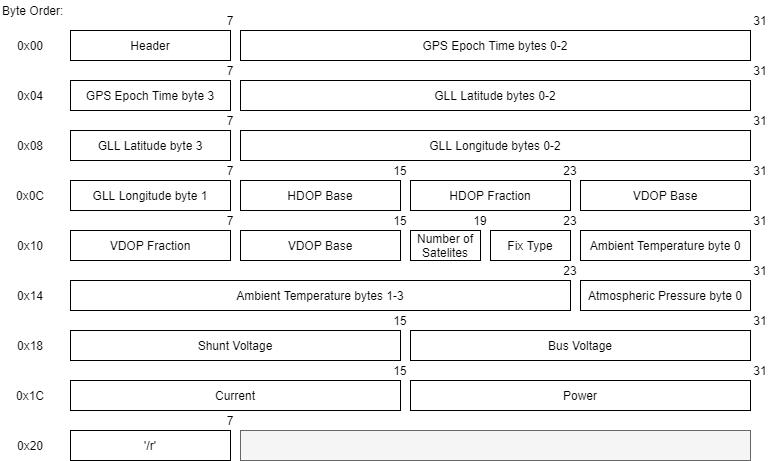
\includegraphics[scale=0.4]{Drift Packet Diagram.png}
	\caption{Diagram showing the structure of a drift data packet including byte position, size and data being collected}
	\label{fig:packet_structure}
\end{figure}

Each Packet begins with a Header. This is an 8-bit value to give information about the data in the payload. This value consist of a 4-bit identifier (0x0 for drift data) as well as a 4-bit number indicating the sample number (1 - 4) before transmission. Data is stored sequentially in little endian format as shown in figure \ref{fig:packet_structure} above. A '\\r' character is used to indicate the end of the packet. This increases the total data requirement from 35 to 37 bytes per sample however, by adding the tail and the header, data integrity is maintained and allow for the standardisation of data transmission.\par  

IMU data however, is of uniform type therefore, no special structures needed to be created. Data from the IMU is stored in an 8-bit buffer array with the most significant byte of the measurement first. Much like the drift buffer, The data was combined into a packet with a header created at the beginning. The header was given the value 0x57 or \textit{"W"} to identify the packet as an IMU data packet. Then the data occupies the remaining bytes with the final byte of the packet assigned to the '<cr>' character to indicate the end of the packet. \par 

Data is stored in the flash chips in packet structure form in the first page of the first available flash chip. Packets are stored sequentially until the device enters transmit state. All data is downloaded from memory and uploaded to the Iridium transmission buffer. The device initiates 2 transmission sessions. First the drift data is uploaded and transmitted, Then the IMU data.Upon successful transmission, the data is sent via satellite network to the Rock7 Rockblock server. The data is saved to a user's account and sent to their email address where the data can be downloaded as an attachment. The diagram below shows the flow of data from the sensors to the user 

\begin{figure}[H]
	\centering
	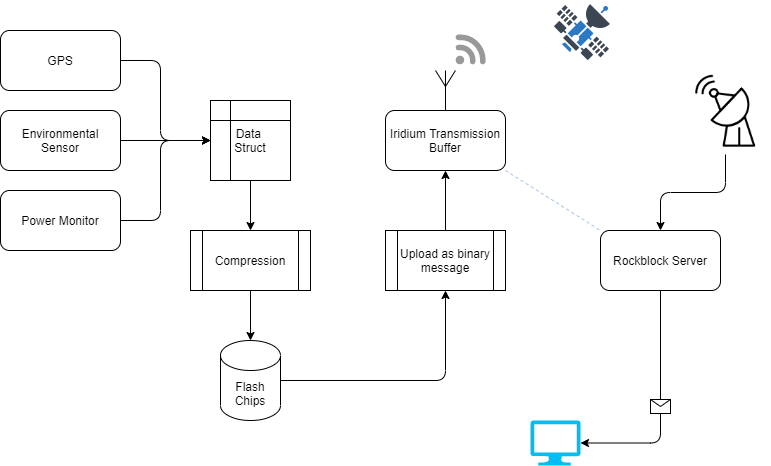
\includegraphics[scale = 0.5]{Data Flow Diagram.png}
	\caption{Diagram showing the flow of data during a cycle of the buoy. The data is sampled by the sensors and converted into packet form where it is stored until it is ready to be transmitted. The transmitted data arrives at a server and is sent via email to the user}
	\label{fig:data_flow}
\end{figure}